\documentclass[uplatex,dvipdfmx]{jsarticle}

%\usepackage{luatexja}
\usepackage{docmute}

%\usepackage[2.0]{bxpdfver}


\usepackage{graphicx}

\usepackage{xcolor}
\graphicspath{{./docs/images/}{./images/}}
\definecolor{forground}{gray}{0.75}
\definecolor{background}{gray}{0.10}
\color{forground}
\pagecolor{background}

\usepackage{siunitx}

\usepackage{tikz}
\usetikzlibrary{intersections,calc,arrows.meta}

%\usepackage[style=base]{caption}
\usepackage[subrefformat=parens]{subcaption}

\usepackage{prettyref}
\newrefformat{note}{脚注~\ref*{#1}}
\newrefformat{figs}{図~\ref*{#1}}
\newrefformat{fig}{図~\ref*{#1}}
\newrefformat{tbl}{表~\ref*{#1}}
\newcommand*{\fullref}[1]{\hyperref[#1]{\prettyref{#1}}}

\usepackage[pdfusetitle,hidelinks]{hyperref}
\usepackage{pxjahyper}

\newcommand*{\includefig}[5][c]{%
    \begin{minipage}[#1]{#2\linewidth}
        \centering
        \includegraphics[width=\linewidth]{#5}
        \subcaption{#3}
        \label{#4}
    \end{minipage}
}
\newenvironment{imageHere}[2][htbp]{\def\@imageHereTmp{#2}%
    \begin{figure}[#1]
        \centering
}{%  
        \caption{\@imageHereTmp}
        \label{figs:\@imageHereTmp}
    \end{figure}
}

\title{
    コズミックトラベル (編集中) \\
    \large 75th2600内装設計チーフ引き継ぎ
}
\author{75th621 千葉森生}
\date{最終更新日: \today}

\begin{document}

\section{内装設計気取りの駄文}

\subsection{第1回プレゼン大会@Jan 13 (原案班)}

我々のクラスでは、数人ずつのグループを作って案を考え、2回のプレゼンを経て最終案を決定しました。

初期の案では、4組が同時に参加できる方式を考えていました。4つの少しずつ異なる部屋を用意して相互に連結し、レールの上を回す、というアイデアです。
ミニゲームについては具体的に決めず、クラスから公募する方針でした。
この段階で、プレゼンに向けてBlenderを用いて3Dモデルを作成しました。
具体的なサイズなどが感覚的にわかるため、これはかなり良かったです。sketchupでも構わないので作るといいと思います。

\begin{imageHere}{原案1}
    \includefig{0.45}{企画書}{fig:企画書}{images/presentation/original_plan.png}
    \includefig{0.45}{3Dモデル}{fig:3Dモデル1}{images/presentation/3D_model/3D_model_1_1.png}
\end{imageHere}

\clearpage

\subsection{第2回プレゼン大会@Feb 10 (原案班)}

十分な耐久性、安定性のあるレールが低コストでは作れない、連結部の耐久性が確保できないなどの理由から、レールを用いた方式を取り止めました。
代わりに採用したのが、成蹊大学の「劇団円想者」\footnote{\url{http://yensosha.blog53.fc2.com/blog-entry-592.html}}がブログに写真を公開していた回り舞台です。この構造なら全て一体型のため連結部やレールが不要で、キャスターのみで回すことができます。
骨組みの基本的な構造は、最後までこれを踏襲しています。
6つのパーツに分かれているため文化祭前の教室復元
    \footnote{\hypertarget{note:教室復元}{教室復元}とは、夏休みと文化祭の間に授業日があったため、そこに向けて内装を一旦解体するイベント。コロナ禍のため平時以上に広いスペースを確保しなければならなかった。幸い、この年の教室復元は最終的になくなり、翌2022年もなかった。今後も復活することはないと思われる。}
でパーツに分けて教室の隅に寄せることができる、補強さえすれば余計なコストをかけずに木材だけで十分な強度が得られることなどが採用理由です。

\begin{imageHere}{原案2-1}
    \begin{minipage}{0.5\linewidth}
        \centering
        \includefig{1}{3Dモデル}{fig:3Dモデル2}{images/presentation/3D_model/3D_model_2_2.png}
    \end{minipage}\hfill
    \begin{minipage}{0.4\linewidth}
        \centering
        \includefig{1}{円想者の舞台(1)}{fig:円想者1}{images/presentation/base_bone_1.jpg}
        \includefig{1}{円想者の舞台(2)}{fig:円想者2}{images/presentation/base_bone_2.jpg}
    \end{minipage}
\end{imageHere}

\begin{imageHere}{原案2-2}
    \includefig{0.45}{スライドの抜粋(1)}{fig:スライド1}{images/presentation/presentation2_1.png}
    \includefig{0.45}{スライドの抜粋(2)}{fig:スライド2}{images/presentation/presentation2_2.png}
    \includefig{0.35}{ミニゲームについて}{fig:ミニゲーム}{images/presentation/minigame.jpg}
    \includefig{0.25}{意見・質問(1)}{fig:質問1}{images/presentation/feedback_1.png}
    \includefig{0.25}{意見・質問(2)}{fig:質問2}{images/presentation/feedback_2.png}
    \includefig{0.45}{意見・質問への解答}{fig:質問3}{images/presentation/feedback_3.png}
\end{imageHere}

\clearpage

\subsection{展示決定@Mar 3}

上記の案で確定し、ストーリーやミニゲームなどの詳細を作り始めました。

このころ、部屋を分けることで無駄な空間が多くなり、各部屋がかなり狭くなってしまうことが判明し、\\一つの箱を2または3個に分割する案に移行しました。

\begin{imageHere}{部屋の分割}
    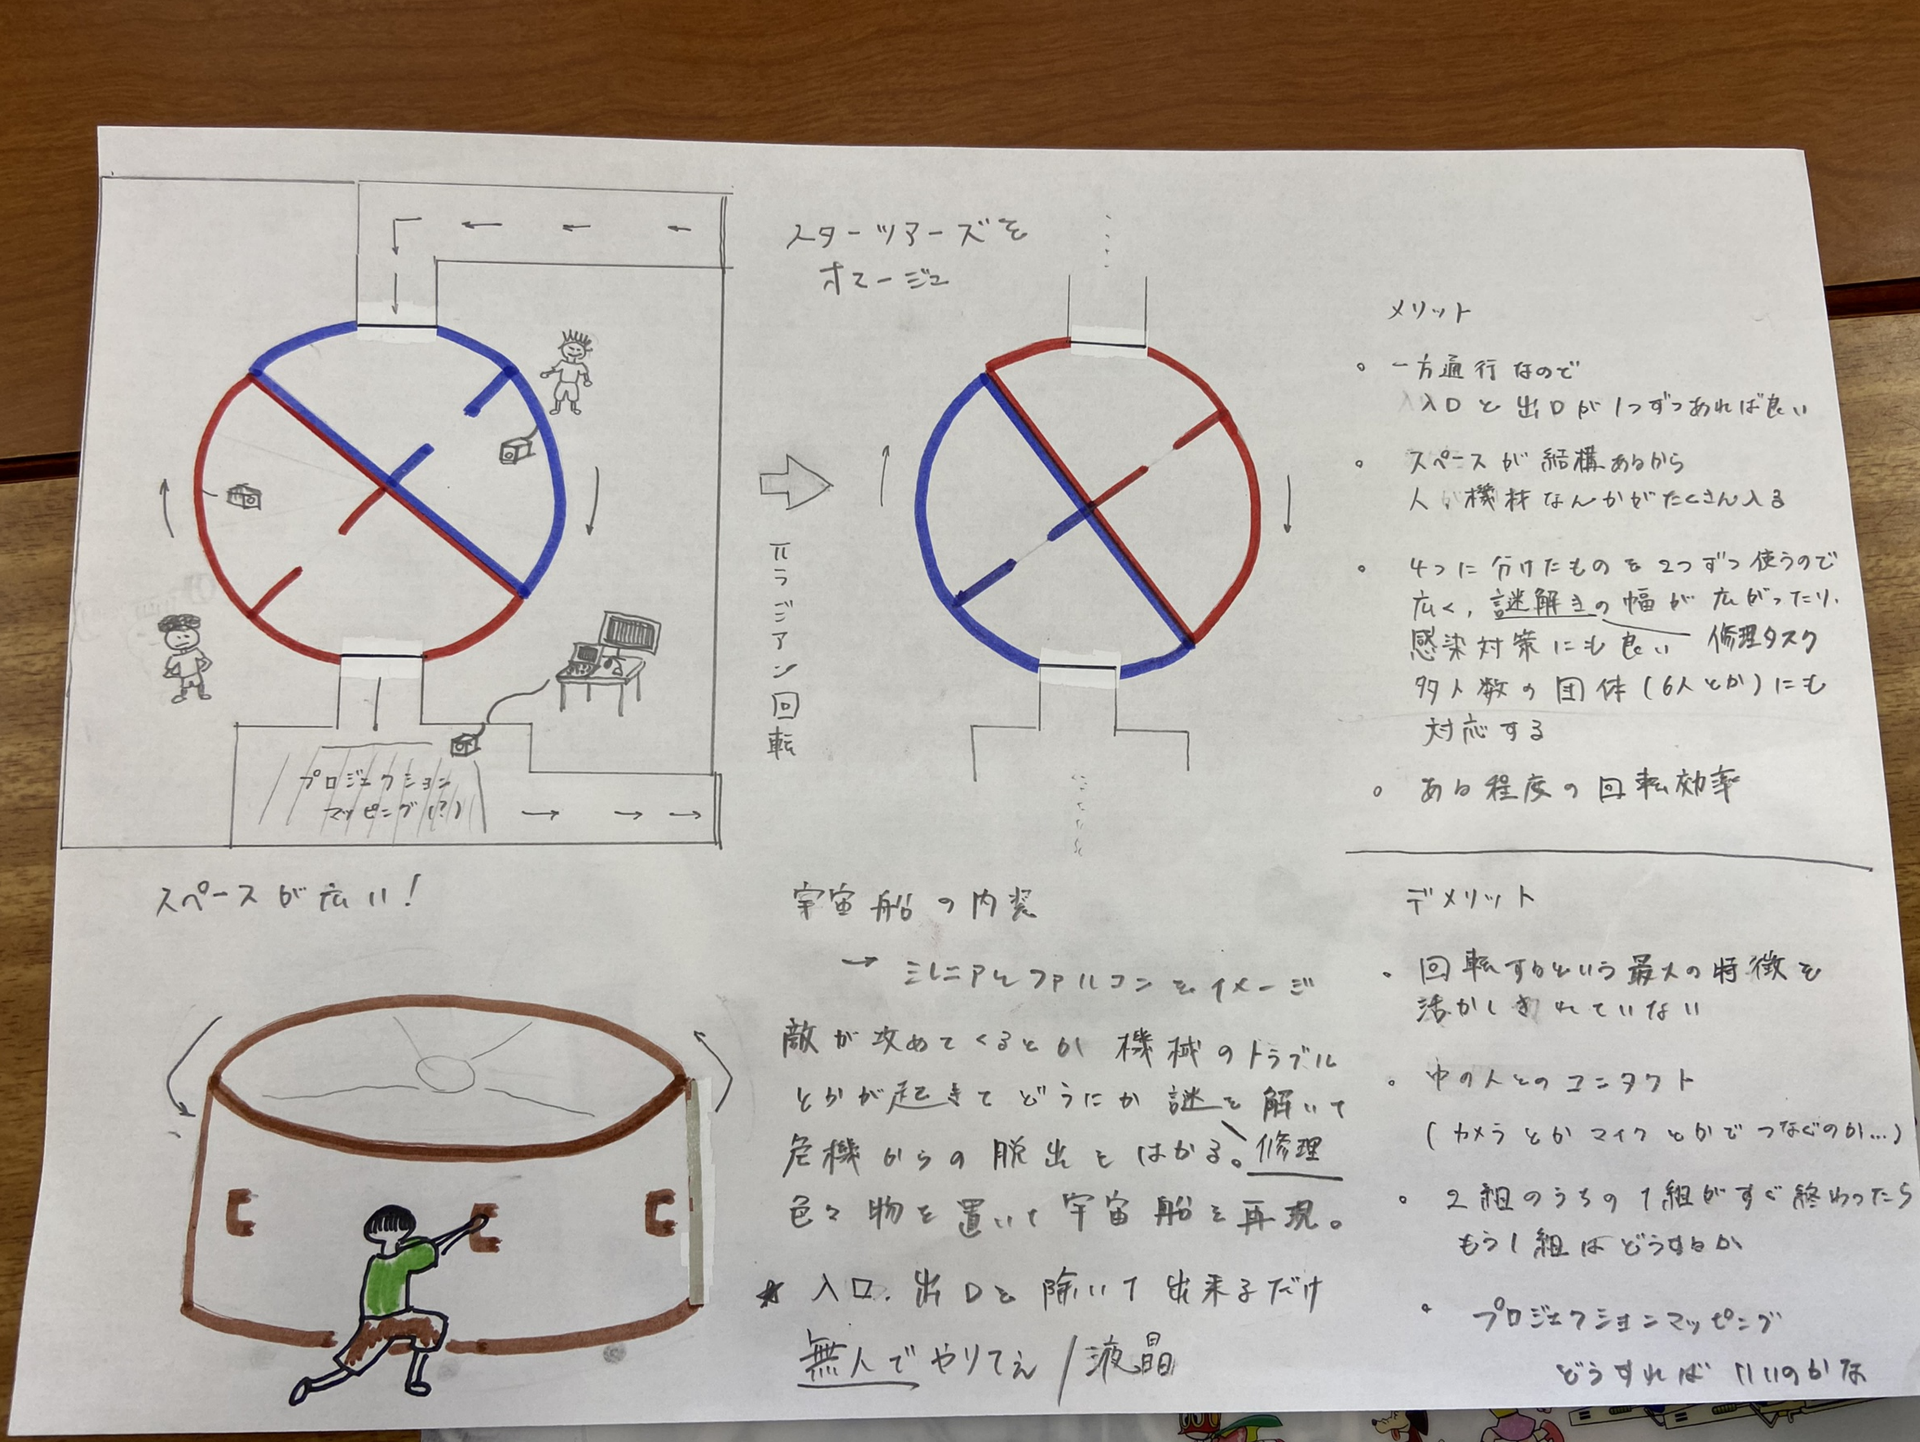
\includegraphics[width=0.7\linewidth]{images/minigame/0.png}
\end{imageHere}

\subsection{ミニゲームプレゼン@Mar 22}

具体的なゲーム内容を決定します。これによって細部の設計、例えば宇宙船外にも構造を作る必要があるのか、タラップの構造はどうするのか、などが決まってきます。
また、デザイン案についても具体的なものが多く出てきたので、ここから本格的な設計の検討が始まりました。

6案が出て、そのうち佐野案(図\ref{figs:ミニゲームプレゼン}\subref{fig:佐野案})では紙で内装の模型(図\ref{figs:ミニゲームプレゼン}\subref{fig:模型1}\subref{fig:模型2})を作ってきてくれました。
実際に宇宙船が回転できるものだったので皆にイメージを持ってもらうためにも一役買い、最後までお世話になった模型になりました。
また、同案の内装のイメージはそのままの再現こそできなかったもの、ドアなどのデザイン・設計の目標となりました。

田中案(図\ref{figs:ミニゲームプレゼン}\subref{fig:田中案})は最終的なストーリーのベースとなりました。
ただ、船外の装飾は時間的制約の関係で実現できず、窓も無くなっています。

\begin{imageHere}{ミニゲームプレゼン}
    \includefig[t]{0.45}{模型-全体像}{fig:模型1}{images/minigame/1.jpg}
    \vspace{-35mm}
    \includefig[c]{0.45}{模型-タラップ}{fig:模型2}{images/minigame/2.jpg}
    \includefig[b]{0.45}{内装イメージ(佐野案)}{fig:佐野案}{images/minigame/3.jpg}
    \includefig[b]{0.45}{船外を装飾する案(田中案)}{fig:田中案}{images/minigame/4.jpg}
\end{imageHere}

\clearpage

\subsection{デザイン開始@May 30}
まずはタラップからデザインが開始しました。なお、設計はとっくに始まっていて、内チに催促しまくってデザイン班を動かしてもらいました。
デザインが完成するのはどうしてもぎりぎりになりがちです。デザインを待ってから設計するという考えは抱かず、後から修正すればいいと思ってどんどん突き進んでしまいましょう。

ちなみにこの段階の設計は、まだsketchupでは作らず、ひたすらに教室の測定と黒板を用いた平面図での設計をもう一人の内設チと一緒に行っていました。緊急時の通路などをふくめゲストの通る可能性のある場所がもれなく文実規則を満たすようにしなければならず、特に宇宙船と壁の間の間隔を確保するための計算が面倒くさかったです。

それから、板パタと書いてあるやつは宇宙船とタラップの間の渡り板のことで、紆余曲折あって最終的に「イカ」と呼ばれるようになっていきます。

\begin{imageHere}{平面図}
    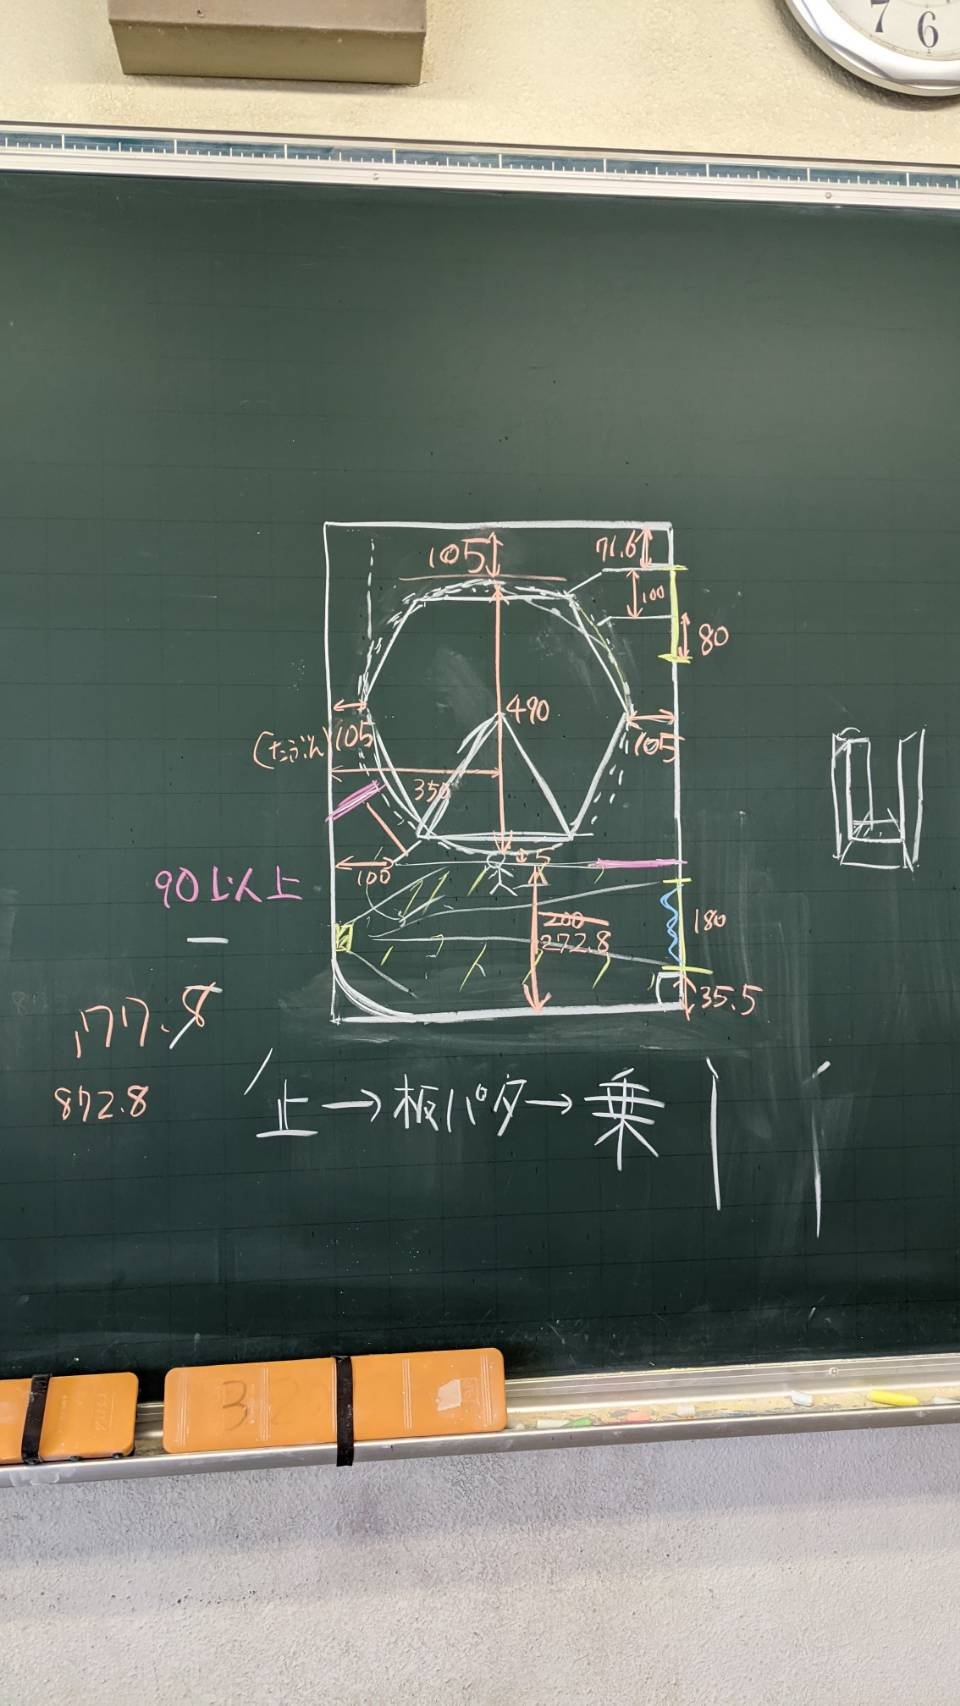
\includegraphics[width=0.45\linewidth]{images/plan/69138.jpg}
\end{imageHere}

\end{document}